\documentclass[a4paper,10pt,journal]{IEEEtran}

% Extension packages providing additional functionality
\usepackage{amsmath}       % additional math environments
\usepackage{graphicx}      % graphics import from external files
\usepackage{epstopdf}      % automates .eps to .pdf conversion
% epstopdf package may require --shell-escape option to pdflatex
\usepackage{booktabs}      % table typesetting additions
\usepackage{siunitx}       % number and units formatting
%\usepackage{caption}       % customisation of captions
\usepackage{url}           % format url addresses
%\usepackage{tikz,pgfplots} % diagrams and data plots

% some handy commands for referencing;
% the optional argument overrides the default label, e.g.
% \figref[FIG.~]{fig:label}
\newcommand{\figref}[2][\figurename~]{#1\ref{#2}}
\newcommand{\tabref}[2][\tablename~]{#1\ref{#2}}
\newcommand{\secref}[2][Section~]{#1\ref{#2}}


\begin{document}

\title{Nanocomposite Design of Thermoelectric Materials\\Introductory
Report}
\author{\IEEEauthorblockN{Callum Vincent}\\
\IEEEauthorblockA{cv235@exeter.ac.uk\\24 November 2013}
}

\IEEEaftertitletext{\vspace{-1\baselineskip}\noindent
%\begin{abstract}
Thermoelectrics are a promising area of materials research recently
revitalised by the introduction of nanocomposites. Obtaining a
thermoelectric figure of merit $ZT > 3$, potent new energy applications
are attainable. Current bulk thermoelectric materials reach $ZT < 1$,
realising practical efficiencies of ~4\%.
Reductions of # in phonon thermal conductivity $kappa_{ph}$ have been
suggested \cite{crc-handbook}, with potential for $ZT > #$. Applying the
Boltzmann transport equation to the phonon and nearly free electron
models for the concept of phonon glass electron crystal (PGEC)
\cite{crc-handbook} we search for a mechanism through which
$kappa_{ph}$ can be reduced. If such a mechanism is discovered, we
will design and computationally model new material structures to
demonstrate its validity.
\end{abstract}

\vspace{1\baselineskip}}

\maketitle

\section{Introduction}

From its discovery in 1821, thermoelectricity has seen constant
attention by the scientific community. Its source lies deep in the
fundamental nature of solid state materials. Through understanding
thermoelectricity we meld all the concepts underpinning solid state
physics; a well defined thermoelectric theory is the culmination of
solid state physics.

%citations below? for the numbers?

Thermoelectricity is not only a central area of research for solid
state physics, but also has enormous practical significance. Current
bulk thermoelectrics achieve thermoelectric figure of merit $ZT$ up to
one, which results in a practical thermal efficiency (heat to work) of
just 4\%, six times less than modern internal combustion engines.
Despite this low figure, thermoelectrics still see niche use
in refrigeration and space exploration due primarily to their
exceptional reliability. By increasing $ZT$ up to three, new
applications in heat recovery systems and solar thermal generators
emerge, improving the thermal efficiency of current power generation
methods. Theoretically, there is no upper limit to $ZT$, and as it
approaches infinity, efficiencies at the Carnot limit can be obtained.
If we achieve $ZT \to\infty$, all heat gradients will be maximally
exploitable for high value electrical energy; once where there were
water wheels, there became hydroelectric dams, now where there is
heat, there will be thermoelectricity.

\section{Thermoelectric Physics}
In 1821, Thomas Seebeck discovered that a circuit made from two
dissimilar metals, with junctions at different temperatures would
deflect a compass magnet (\figref{seebeck-experiment}), he had
discovered thermoelectricity. The temperature gradient $\nabla
T$ between the junctions generates an electromotive force:

\begin{equation}
\label{seebeck-emf}
	E_{emf} = -S \nabla T
\end{equation}
where $S$ is the Seebeck coefficient, defined as the induced voltage per
unit temperature $S = \frac{\Delta V}{\Delta T}$. This coefficient is
not only material dependent, but also temperature dependent, i.e., a
temperature gradient produces an electromotive force gradient. This
electromotive force gradient produces a current density gradient
described macroscopically by a modified ohms law:

\begin{equation}
\label{current-density}
	J = \sigma (-\nabla V - S \nabla T)
\end{equation}
where $J$, $V$ and $\sigma$ are the current density $\frac{I}{A}$,
voltage and electrical conductivity at a given location in the
material. If we were to repeat the experiment conducted by Seebeck
(\figref{seebeck-experiment}), using a probe to measure the varience
of $J$, $V$ and $\sigma$ across one of the metals would give the
Seebeck coefficient.
For the purposes of our project, we will be deriving an expression for
the Seebeck coefficient from the microscopic ohms law:

\begin{equation}
\label{micro-ohm}
	J = \frac{ne^2E \tau}{m_e}
\end{equation}
where $n$ is the density of free electrons in the material, $e$ is
elementary charge, $E$ is the electric field accelerating the
electrons, $\tau$ is the mean time between the electron colliding with
something in the material and $m_e$ is the electron mass.


\begin{figure}
	\centering
	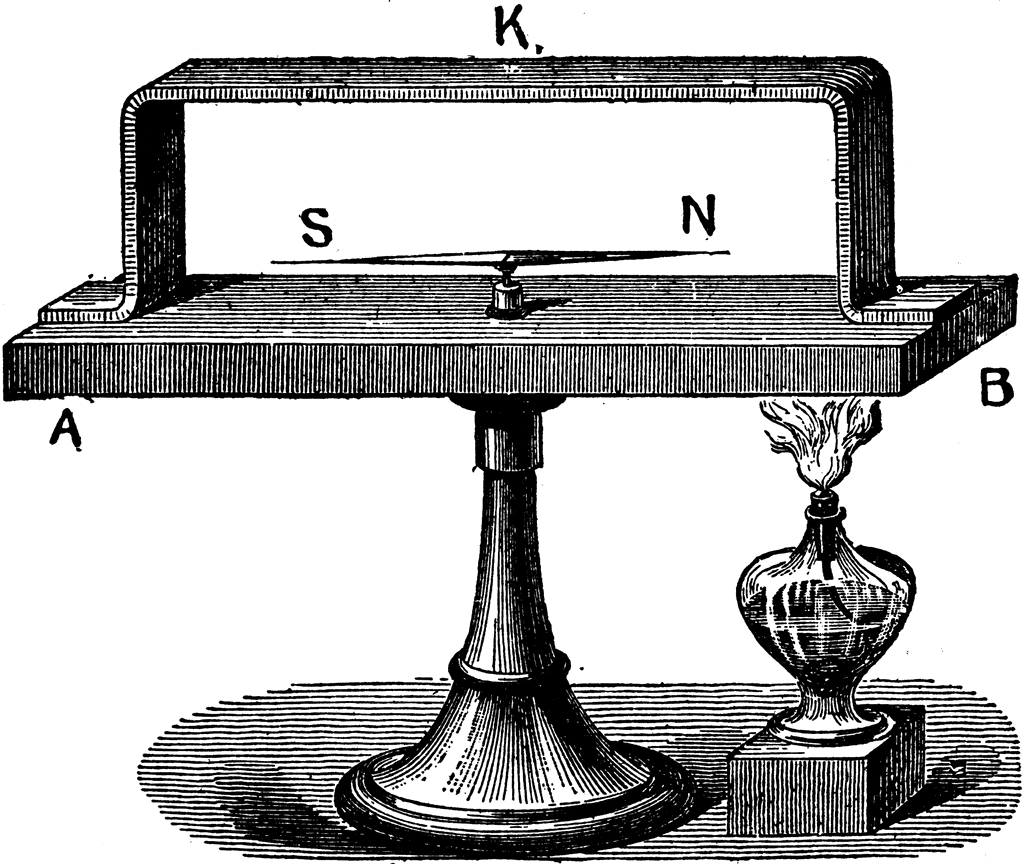
\includegraphics[width=0.5\textwidth]{seebeck-experiment-black.png}
	\caption{Thomas Seebeck's original thermoelectricity experiment
	diagram \cite{seebeck-original}. Bridge of metal (K), above a compass
	needle on top of a different metal heated at one side.}
	\label{seebeck-experiment}
\end{figure}

Thermoelectricity, its uses and current research is well summarised by
J. W. Bos \cite{rsc-eic}.

\section{Models and Assumptions}
For our project we will be using the nearly free electron model, which
assumes no electron-electron interactions

\bibliographystyle{IEEEtran}
\begin{thebibliography}{2}
\bibitem{crc-handbook}
D. M. Rowe, \emph{CRC Handbook of Thermoelectrics}. CRC Press, 1995
\bibitem{rsc-eic}
J. W. Bos, \emph{Thermoelectric materials: efficiencies found in
nanocomposites}. Education in Chemistry, March 2012. [Online] Available
from:
\url{http://www.rsc.org/images/Thermoelectric-materials_tcm18-214041.pdf} [Accessed 24 November 2013].
\bibitem{seebeck-original}
\url{etc.usf.edu/clipart/35600/35659/seebeck_35659_lg.gif 24 November
2013
\end{thebibliography}

\end{document}